\documentclass[11pt,xcolor={dvipsnames},aspectratio=159,hyperref={pdftex,pdfpagemode=UseNone,hidelinks,pdfdisplaydoctitle=true},usepdftitle=false]{beamer}
\usepackage{presentation}[aspectratio=169]
\usepackage{math}
\usepackage{mathtools}
\usepackage{amsmath}
\usepackage{mleftright}

% Enter title of presentation PDF:
\hypersetup{pdftitle={Seignorage and inflation}}
% Enter link to PDF file with figures:


\begin{document}
% Enter presentation title:
\title{Seignorage and inflation}
\subtitle{Fiscal and Monetary Policy 2024}
% Enter presentation information:

% Enter presentation authors:
\author{Piotr Żoch}%
% Enter presentation location and date (optional; comment line if not needed):
\frame{\titlepage}

% Fill out content of presentation:
\begin{frame}{Budget constraint again}
    \begin{itemize}
    \item To link deficits and debt with monetary policy we revisit the intertemporal government budget constraint.
    \item The static budget constraint of the \al{fiscal branch} of the government is \begin{align*}
       P_t G_t + i_{t-1} B^T_{t-1} = P_t T_t + \bp{B^T_t-B^T_{t-1}} + RCB_t
    \end{align*}
    where $i_t$ is the nominal interest rate promised at $t$, $B^T_t$
    is total \alb{nominal} debt issued in period $t$, $G_t$ is real government purchases, $T_t$
    is real (net) tax revenue and $RCB_t$ is direct receipts from the
    central bank.
    \end{itemize}
\end{frame}

\begin{frame}{Budget constraint again}
    \begin{itemize}
    \item The central bank has a similar budget constraint: 
    \begin{align*}
        B^M_t - B^M_{t-1} + RCB_t = i_{t-1} B^M_{t-1} + \bp{M_t - M_{t-1}}.
    \end{align*}
    where $B^M_t$ is the central bank's purchases of government debt, and
    $M_t - M_{t-1}$ is an increase in nominal money supply in period t.
    \item $M_t$ here is high-powered money, monetary base --  stock of currency held by the nonbank public + bank reserves.
    \end{itemize}
\end{frame}

\begin{frame}{Budget constraint again}
    \begin{itemize}
    \item \al{If} we do not put any restriction on $RCB_t$, then we can add the two budget constraints to obtain \begin{align*}
        P_t G_t + i_{t-1} B_{t-1} = P_t T_t + \bp{B_t-B_{t-1}} + \bp{M_t - M_{t-1}}.
    \end{align*}
    \item It makes clear that the government can finance its spending needs by issuing debt or by printing money.
    \item Does the liability composition matter? The only difference is that debt pays interest. 
    \end{itemize}
\end{frame}

\begin{frame}{Budget constraint again}
    \begin{itemize}
    \item In real terms:  \begin{align*}
         G_t + \bar{r}_{t-1} \frac{B_{t-1}}{P_{t-1}} = T_t + \bp{\frac{B_t}{P_t}-\frac{B_{t-1}}{P_{t-1}}} + \bp{\frac{M_t}{P_t} - \frac{1}{1+\pi_t} \frac{M_{t-1}}{P_{t-1}}}.
    \end{align*} where $1+\pi_t \coloneq \frac{P_t}{P_{t-1}}$ and $1+\bar{r}_{t-1} \coloneq \frac{1+i_{t-1}}{1+\pi_t}$.
    \item Here $\bar{r}_{t-1}$ is the \al{ex post} real interest rate on government debt.
    \item \al{Unanticipated} inflation reduces the real value of debt.
    \end{itemize}
\end{frame}

\begin{frame}{Monetary financing}
    \begin{itemize}
    \item Real resources due to monetary financing are \begin{align*}
        S_t \coloneq \frac{M_t}{P_t} - \frac{1}{1+\pi_t} \frac{M_{t-1}}{P_{t-1}}.
    \end{align*}
    \item We call this the \alb{seigniorage} revenue.
    \item It can be rewritten as \begin{align*}
        \frac{M_t}{P_t} - \frac{M_{t-1}}{P_{t-1}} + \frac{\pi_t}{1+\pi_t} \frac{M_{t-1}}{P_{t-1}}. 
    \end{align*}
    \item Two sources of seignorage:
    \begin{enumerate}
        \item change in real money holdings;
        \item to maintain constant real money holdings the private sector needs to purchase more nominal money to offset the effects of inflation.
    \end{enumerate}
    \end{itemize}
\end{frame}

\begin{frame}{Monetary financing}
    \begin{itemize}
    \item Are there limits to monetary financing? 
    \item Study the formula in the steady state: \begin{align*}
        G + r \frac{B}{P} = T + \frac{M}{P} \frac{\pi}{1+\pi}.
    \end{align*}
    \item Is it possible to finance \al{any real government purchases} by printing money?
    \item The answer depends on $\frac{M}{P} \frac{\pi}{1+\pi}$
    \item In most models demand for \alg{real} balances $\frac{M}{P}$ is decreasing in the nominal interest rate (so also in inflation).
    \item The other term is increasing in inflation, but bounded by 1.
    \item A Laffer curve for inflation?
    \end{itemize}
\end{frame}

\begin{frame}{}
    \begin{figure}
        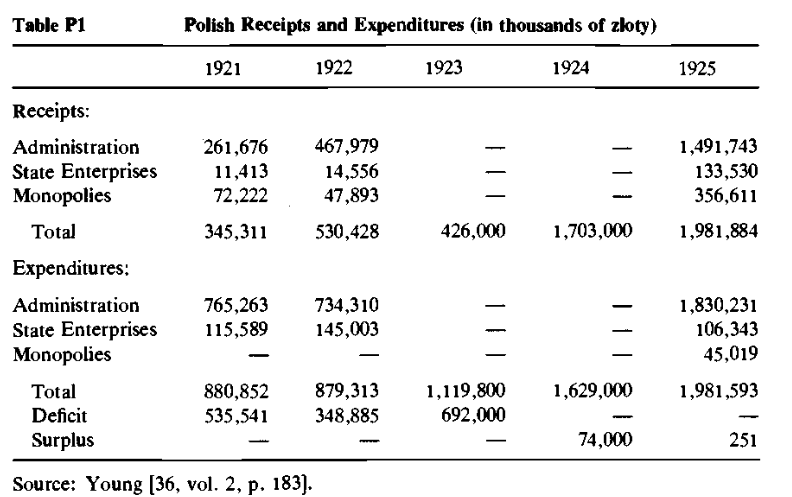
\includegraphics[width=0.8\textwidth]{sargent1.png}
        \caption{Sargent (1982)} 
    \end{figure}
\end{frame}

\begin{frame}{}
    \begin{figure}
        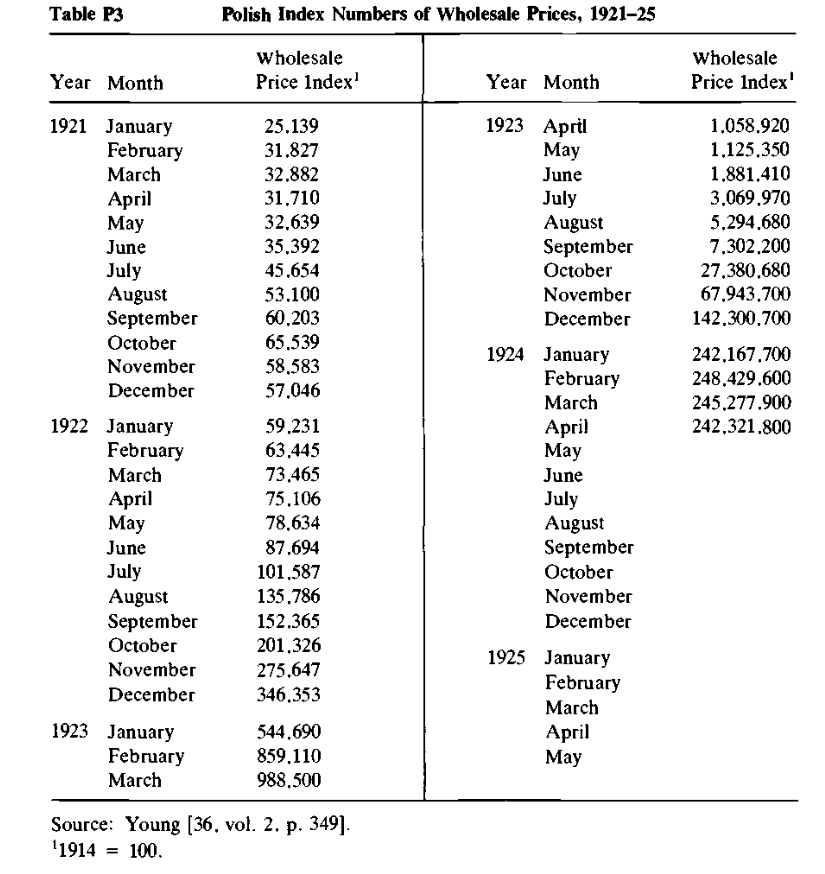
\includegraphics[width=0.5\textwidth]{sargent2.png}
    \end{figure}
\end{frame}

\begin{frame}{Monetary financing}
    \begin{itemize}
    \item Can the government boost demand for real balances?
    \item Restrictions on the rights of banks and other intermediaries to issue close substitutes for government issued currency.
    \item Limitations on trading assets that are close substitutes for government issued currency.
    \item Reserve requirements. 
    \item At the end of the day it amounts to a transfer of real resources from the private sector to the government -- is it any different from taxation?
    \end{itemize}
\end{frame}

\begin{frame}{Monetary financing}
    \begin{itemize}
    \item What is the \alb{optimal} level of seignorage? 
    \item Without a fully specified model it is hard to say, but we can think about the tradeoffs.
    \item Note that inflation is like a distortionary tax on money holdings.
    \item But other taxes (consumption, capital, labor) are usually distortionary too.
    \item This is an argument for \al{some positive} inflation -- distortion smoothing.
    \end{itemize}
\end{frame}

\begin{frame}{Detour: optimal quantity of money?}
    \begin{itemize}
    \item Friedman's (1969) discussion of the optimal quantity of money is related to this. 
    \item Suppose the government can levy a non-distortionary tax on the private sector. How much money should it print?
    \item In this case fiscal considerations are irrelevant.  
    \item The optimum calls for the government to print money until the marginal benefit of money equals the marginal cost.
    \end{itemize}
\end{frame}

\begin{frame}{Detour: optimal quantity of money?}
    \begin{itemize}
    \item The opportunity cost of holding money is the nominal interest rate.
    \item At the optimum money and bonds should be perfect substitutes: nominal interest rate should be zero.
    \item Because $i = r + \pi$, this implies that inflation should be constant and equal to the negative of the real interest rate.
    \item If $r>0$ then the optimal inflation rate is negative. 
    \item \alb{Friedman's rule}: satiate the demand for money.
    \end{itemize}
\end{frame}

\begin{frame}{Limits of monetary policy?}
    \begin{figure}
        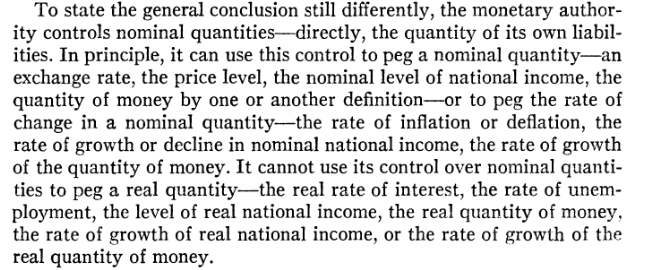
\includegraphics[width=1\textwidth]{friedman1968.png}
        \caption{Friedman (1968)} 
    \end{figure}
\end{frame}

\begin{frame}{Limits of monetary policy?}
    \begin{itemize}
        \item Friedman (1968) warned not to expect too much from monetary
        policy.
        \item He argued that a monetary authority \al{could exert substantial
        control} over the inflation rate, especially in the long run.
        \item Is it really true? What assumptions are needed to ensure that?
        \item Recall that there is an equation that links debt, deficits, and inflation. 
        \item We will tackle this question in two ways:
            \begin{enumerate} \item 
                first illustrate the idea in an environment with money (Sargent and Wallace, 1981);
                \item then reconsider the role of the government budget "constraint"
            \end{enumerate}
    \end{itemize}
\end{frame}

\begin{frame}{Some Unpleasant Monetarist Arithmetic}
    \begin{itemize}
        \item Sargent and Wallace (1981) warn us about thinking about monetary policy and fiscal policy separately.
        \item They study a simple endowment economy with money.
        \item The nominal government budget constraint is \begin{align*}
            B_t + M_t = P_t \bp{G_t - T_t} + \bp{1+i_{t-1}} B_{t-1} + M_{t-1}.
        \end{align*}
        \item Demand for real balances decreases in the nominal rate \begin{align*}
            \frac{M_t}{P_t} = L\of{i_t} \end{align*}
        \item The Fisher equation is \begin{align*}
            1 + i_t =\bp{1+r_t}\bp{1+\pi_{t+1}} \end{align*}
    \end{itemize}
\end{frame}


\begin{frame}{Some Unpleasant Monetarist Arithmetic}
    \begin{itemize}
        \item Let $B_{-1},M_{-1}$ and $i_{-1}$ be given and assume that $r_t = r$. 
        \item Assume the IGBC is satisfied to obtain \begin{align*}
            \sum_{t=0}^\infty \bp{\frac{1}{1+r}}^t \frac{M_t - M_{t-1}}{P_t} =  \sum_{t=0}^\infty \bp{\frac{1}{1+r}}^t \bp{G_t - T_t} + \frac{B_{-1}}{P_0}\bp{1+i_{-1}}
        \end{align*}
        \item The left hand side is the present value of seignorage. It can be written as 
        \begin{align*}
            \sum_{t=0}^\infty \bp{\frac{1}{1+r}}^t \frac{i_{t-1}}{1+i_{t-1}} L\of{i_t} - \omega L\of{i_{0}}
        \end{align*}
        where $\omega$ is a constant. 
    \end{itemize}
\end{frame}

\begin{frame}{Some Unpleasant Monetarist Arithmetic}
\begin{itemize}
        \item We can write the IGBC as \begin{align*}
            \sum_{t=0}^\infty \bp{\frac{1}{1+r}}^t \frac{i_{t-1}}{1+i_{t-1}} L\of{i_t} - \omega L\of{i_{0}} = D  
        \end{align*}
        \item \al{Key assumption}: the fiscal authority commits to a particular $D$. It will not adjust. 
        \item The monetary authority has to provide financing such that the IGBC holds. 
        \item This means that the monetary authority can \al{only} change the timing of $i_t$ and thus of seignorage revenue.
    \end{itemize}
\end{frame}


\begin{frame}{Some Unpleasant Monetarist Arithmetic}
    \begin{itemize}
            \item Example: the central bank reduces the growth rate of money in early periods to "control inflation".
            \item But it will have to compensate for it with a higher growth rate of money and inflation later on. 
            \item Note: as usually in frictionless models, here higher inflation is associated with \alr{higher} nominal rates.
            \item Conclusion: monetary policy ultimately cannot control inflation, if it is forced to finance deficits. 
        \end{itemize}
    \end{frame}

\begin{frame}{Some Unpleasant Monetarist Arithmetic}
    \begin{itemize}
            \item Sargent and Wallace (1981) provide an even more drastic example. 
            \item Suppose MP is tight initially. It is expected it will be loosened to finance a deficit in the future.
            \item This means high inflation in the future. 
            \item This means high nominal rates in the future.
            \item High nominal interest rates in the future lower demand for real balances today
            \item Given nominal money supply, this means high price level today.
            \item Conclusion: MP tries to control inflation, but actually causes it!
        \end{itemize}
    \end{frame}


\begin{frame}{Some Unpleasant Monetarist Arithmetic?}
    \begin{itemize}
            \item Andolfatto (2021) uses a similar logic to question conventional wisdom about Volcker Disinflation.
            \item Standard narrative: after prolonged inflation in the 1970s, Volcker tightened monetary policy to reduce inflation. This demonstrated that MP can control inflation.  
            \item Andolfatto suggests it was the fiscal policy that was responsible for the disinflation. 
            \item By increasing interest expenses on the debt, Volcker forced the Treasury to reduce deficits.
        \end{itemize}
    \end{frame}

\begin{frame}{Some Unpleasant Monetarist Arithmetic?}
    \begin{figure}
        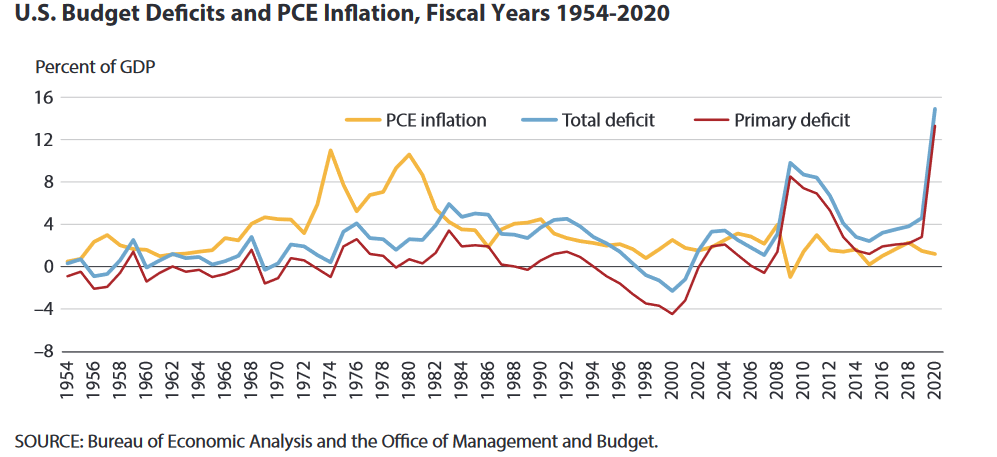
\includegraphics[width=1\textwidth]{andolfattio1.png}
        \caption{Andolfatto (2021)} 
    \end{figure}
\end{frame}

\begin{frame}{Just ``printing money''?}
    \begin{itemize}
            \item So far we have seen that fiscal policy can affect inflation / price levels by affecting supply / demand of money. 
            \item Is there any other link? In particular, what if the economy is \al{cashless}?
            \item We will explore price determination in a more general model next time.  
        \end{itemize}
    \end{frame}


\end{document}